\documentclass[11pt,twocolumn]{article}

% Packages
\usepackage[utf8]{inputenc}
\usepackage[T1]{fontenc}
\usepackage{graphicx}
\usepackage{booktabs}
\usepackage{amsmath}
\usepackage{hyperref}
\usepackage[margin=0.85in]{geometry}
\usepackage{natbib}
\usepackage{caption}
\usepackage{subcaption}
\usepackage{xcolor}
\usepackage{float}
\usepackage{enumitem}
\usepackage{microtype}

\setlength{\columnsep}{0.3in}
\raggedbottom

\title{\textbf{The Shifting Lexicon of American Power:\\Computational Analysis of Political Language\\in State of the Union Addresses, 1950--2026}}

\author{Calder Katyal\\
\text{Yale University}\\
\text{HUMS 3210 (Culture as Data: Thinking Computationally with Text)}\\
\texttt{calder.katyal@yale.edu}}

\date{Spring 2026}

\begin{document}
\maketitle

% ===========================================================================
\begin{abstract}
\noindent This paper uses computational text analysis on a corpus of 79 State of the Union addresses delivered by Presidents from 1950 through 2026, spanning fifteen presidencies from Truman through Trump's second term. Using TF-IDF differential analysis, LDA topic modeling, supervised classification (Linear SVM), and t-SNE document embeddings, we find that (1) the language of the SOTU has changed dramatically over time, tracking shifts in geopolitical and domestic challenges; (2) Democratic and Republican presidents employ measurably different rhetorical vocabularies, with a Linear SVM classifier achieving 92.4\% cross-validated accuracy in distinguishing party from text alone; and (3) proximity in time is at least as strong an organizing principle in the embedding space as party affiliation. The central argument is that the language of the State of the Union is shaped more by the historical moment a president inhabits than by the party to which the president belongs.
\end{abstract}

% ===========================================================================
\section{Introduction}

The State of the Union address occupies a unique place in the American archive of political language. Mandated by Article~II, Section~3 of the U.S. Constitution, it is one of the few textual artifacts created over such a long time span under nearly identical institutional requirements: a single voice (the president) addressing a relatively constant audience (Congress and, in the television era, the nation), with repeated opportunities to deliver a common message. Because of this consistency in format, the SOTU corpus is an unusually controlled object for studying how American political vocabulary has changed---and how those changes reflect the relationship between rhetoric and history.

This paper asks three questions. First, how does the vocabulary of SOTU addresses change across the period 1950--2026? Second, do Democratic and Republican presidents use discernibly different vocabularies? Third, how well can the methods of computational text analysis---what Moretti \citep{moretti2013} calls ``distant reading''---capture these patterns, and where do they fall short? Because these methods rely on abstraction and generalization, they may have blind spots or limitations when identifying certain forms of variation.

The methodology here draws on multiple techniques: vector semantics (TF-IDF), generative topic modeling (LDA), supervised machine learning, and dimensionality reduction for visualization. Following Underwood's \citeyearpar{underwood2019} claim that ``computational methods can uncover patterns that are invisible to human readers working at the level of individual texts,'' each speech is treated as a document within a corpus and analyzed via distributional methods to detect significant temporal shifts and partisan divergences. At the same time, we take seriously the warnings of Drucker \citeyearpar{drucker2017} and D'Ignazio and Klein \citeyearpar{dignazio2020}, who point out that data visualizations and quantitative methods always assume something about what is being counted, what can be compared, and what is hidden from view in the act of abstraction.

% ===========================================================================
\section{Data Curation and Preprocessing}

\subsection{Assembling the Corpus}

Although every corpus may be interpreted differently, we think it is worth describing the decision-making process behind how we built this one. The corpus contains 79 speeches given by 15 U.S. presidents who were in office between 1950 and 2026. The 73 speeches from 1950 through 2020 come from the \texttt{stdlib-js/datasets-sotu} dataset, a GitHub repository drawing on data from the American Presidency Project at the University of California, Santa Barbara. We also collected four addresses from President Joe Biden (2021--2024) and two from President Donald J. Trump's second term (2025--2026); these were gathered directly from the American Presidency Project (\texttt{presidency.ucsb.edu}), where each speech is published as a complete transcript with both the president's remarks and audience reactions noted inline.

Our use of two different sources introduced a small difference in approach. The \texttt{stdlib-js} dataset had virtually no edits made to it, while the transcripts from the Presidency Project contained stage directions (e.g., ``[Laughter]'', ``[Applause]'') alongside the president's remarks. While we could have cleaned the datasets to remove the performative aspects of each document, we chose not to, since doing so risks erasing contextual information about how those statements were received. Stage directions account for approximately 2\% of total tokens, and our document-frequency thresholds filter out most of them, so retaining them has little-to-no effect on the results.

Our decision to begin in 1950 reflects both pragmatic and analytical considerations. Before the mid-twentieth century, SOTU addresses were almost exclusively written messages sent to Congress---a fundamentally different genre from the televised oral address that became standard after Truman. Beginning in 1950 lets the corpus capture a relatively coherent rhetorical form, even as that form evolves from radio-era formality to the applause-punctuated cadences of contemporary addresses.

\begin{table}[h]
\centering
\small
\caption{SOTU Corpus Summary by President}
\label{tab:corpus}
\begin{tabular}{lccr}
\toprule
\textbf{President} & \textbf{Party} & \textbf{Years} & \textbf{$N$} \\
\midrule
Truman & D & 1950--53 & 4 \\
Eisenhower & R & 1953--61 & 9 \\
Kennedy & D & 1961--63 & 3 \\
Johnson & D & 1964--69 & 6 \\
Nixon & R & 1970--74 & 5 \\
Ford & R & 1975--77 & 3 \\
Carter & D & 1978--81 & 4 \\
Reagan & R & 1982--88 & 7 \\
G.H.W.\ Bush & R & 1989--92 & 4 \\
Clinton & D & 1993--2000 & 8 \\
G.W.\ Bush & R & 2001--08 & 8 \\
Obama & D & 2009--16 & 8 \\
Trump (1st) & R & 2017--20 & 4 \\
Biden & D & 2021--24 & 4 \\
Trump (2nd) & R & 2025--26 & 2 \\
\midrule
\textbf{Total} & & & \textbf{79} \\
\bottomrule
\end{tabular}
\end{table}

As Table~\ref{tab:corpus} summarizes, the corpus includes 37 Democratic speeches and 42 Republican speeches---a modest imbalance reflecting the distribution of presidential terms across this period. Each speech averages about 6,014 words in length, but there is substantial variation: Carter's 1981 written message exceeds 33,000 words, while Nixon's 1973 written message (a brief, formally written report presented at the beginning of his second term) is fewer than 1,700. This variation is itself analytically significant, since it reflects the persistence of written policy documents alongside oral oratory throughout the postwar period.

\subsection{Preprocessing Pipeline}

All speeches were first tokenized using NLTK's \texttt{word\_tokenize} function and converted to lowercase. For content-word analyses, stopwords were removed using the NLTK English stopword list. For TF-IDF and topic modeling, we kept both unigrams and bigrams, applied a minimum document frequency of 3 and a maximum document frequency of 90\%, and limited the vocabulary to 5,000 features. These parameters are typical for computational text analysis \citep{jockers2013}, balancing vocabulary coverage against noise. Sentence-level statistics (average sentence length and type-token ratio) were computed using NLTK's \texttt{sent\_tokenize} prior to stopword removal, in order to preserve the syntactic structure of the original text.

% ===========================================================================
\section{Methods and Results}

\subsection{Lexical Trends Over Time}

We begin with what might be called the material history of the SOTU address: how its length and lexical texture have changed over seven decades.

\begin{figure}[H]
\centering
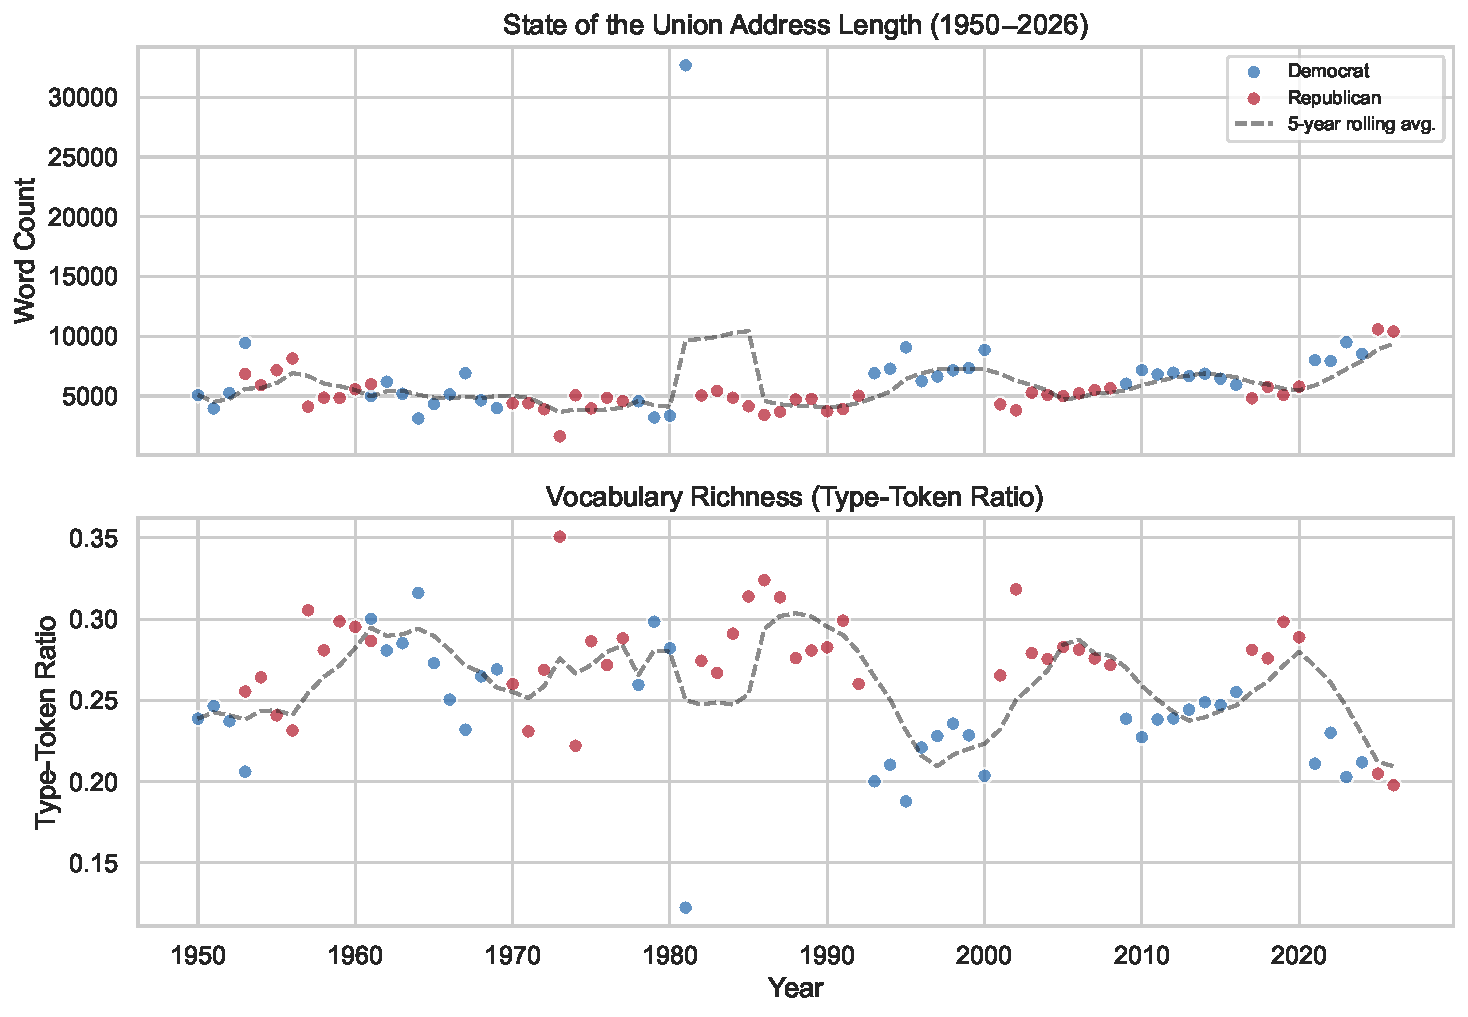
\includegraphics[width=\columnwidth]{figures/fig1_speech_length.pdf}
\caption{Speech length (word count) and type-token ratio, 1950--2026. Points colored by party; dashed line shows a 5-year rolling average.}
\label{fig:length}
\end{figure}

Two distinct trends are apparent in Figure~\ref{fig:length}. First, speech length oscillates rather than declines: most decades cluster in a range of approximately 4{,}000 to 7{,}000 words, the 1970s mark a trough ($\approx$ 4{,}100), and the 1980s mean is inflated by Carter's 33{,}558-word written message of 1981, delivered after he had lost re-election. The striking departure comes at the end of the period: Biden's later addresses (2023--2024) and Trump's two second-term addresses (2025--2026) are among the longest in the corpus---ranging from roughly 8{,}500 to 10{,}700 words---and the 2020s mean of 8{,}760 words is the greatest of any decade. (This expansion is far too large to be attributed to the inclusion of stage directions in post-2020 transcripts, which constitute well under 1\% of tokens.) Second, contrary to a familiar narrative about ``richer'' modern political speech, the type-token ratio does \textit{not} rise across the period. After peaking in the 1960s--80s (mean TTR $\approx 0.275$), vocabulary diversity drops in the 1990s, recovers somewhat in the 2000s, and reaches its lowest values in the 2020s ($\approx 0.221$). Aggregated across the full corpus, Republican speeches exhibit higher type-token ratios than Democratic ones (0.277 vs.\ 0.240), though the pattern is not uniform across decades---in the 1970s and the 2020s, Democratic and Republican TTRs are roughly comparable.

\subsection{Partisan Language: Differential TF-IDF}

To identify the words that characterize each party, we used TF-IDF (term frequency--inverse document frequency) vectorization. We computed TF-IDF vectors for each speech individually and then averaged the resulting feature vectors by party, rather than treating the corpus as a single data point per party. This per-speech averaging strategy gives us an aggregate measure of each party's signature vocabulary without letting the longer addresses of Carter and Truman dominate the signal. Figure~\ref{fig:tfidf} shows the top 20 most discriminating terms for each party.

\begin{figure}[H]
\centering
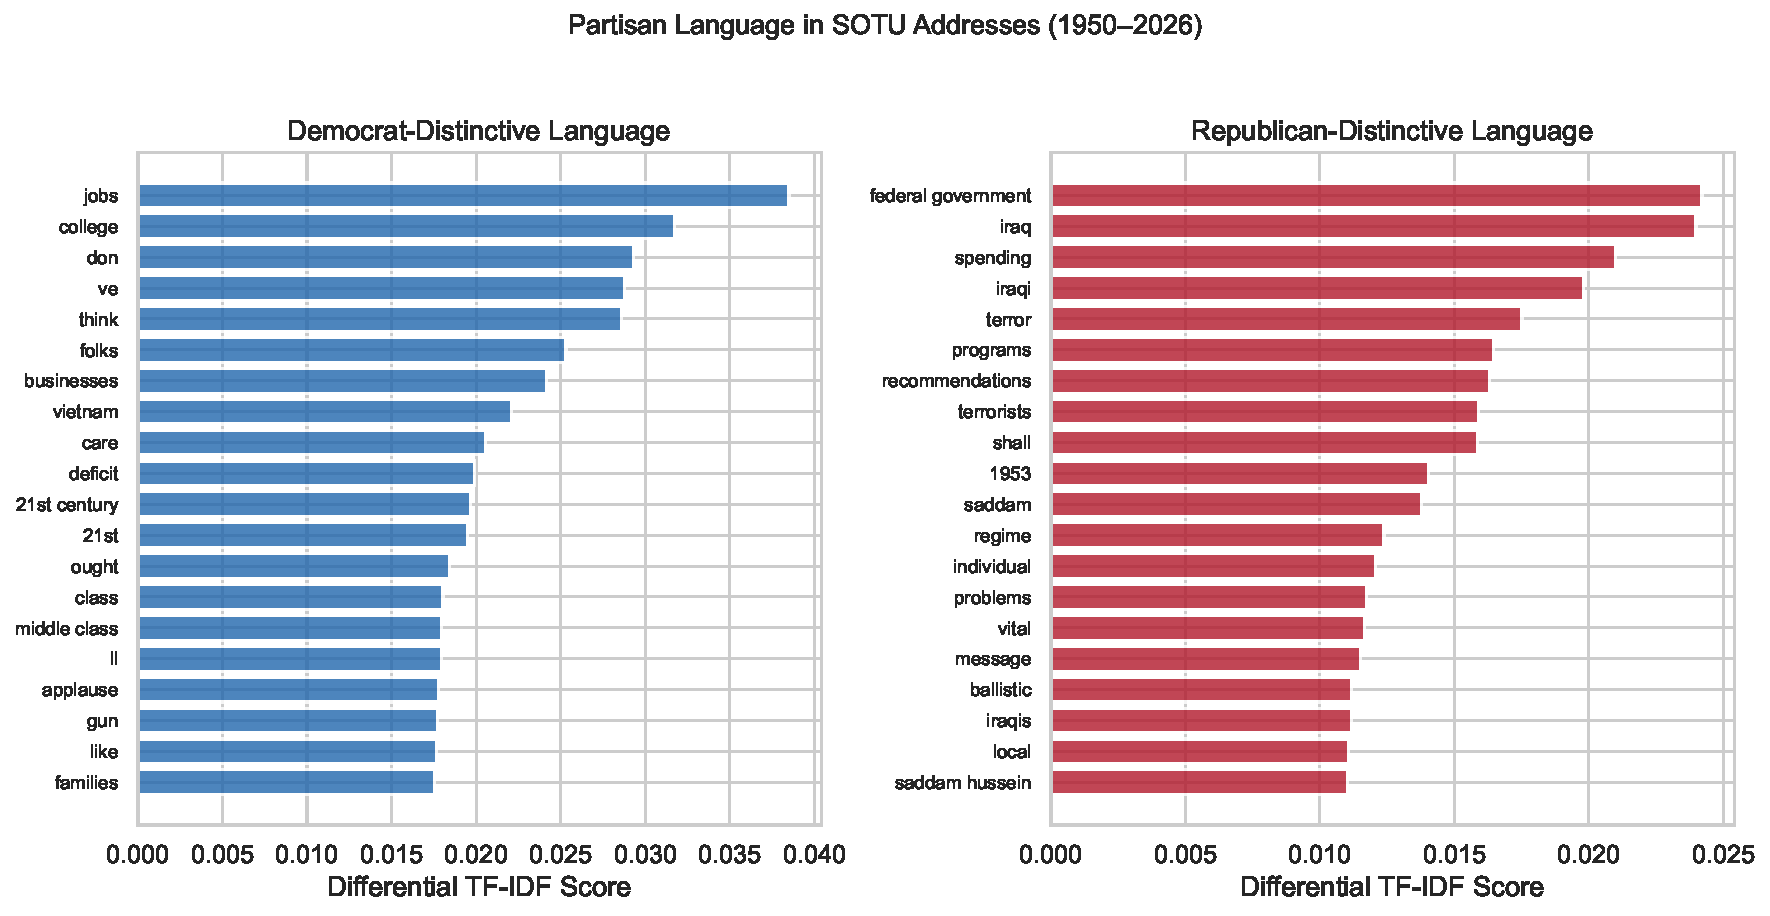
\includegraphics[width=\columnwidth]{figures/fig2_partisan_tfidf.pdf}
\caption{Top 20 terms by differential TF-IDF score for each party. Higher scores indicate stronger association with that party's speeches.}
\label{fig:tfidf}
\end{figure}

The word lists are immediately legible as partisan vocabularies. The terms that characterize Republicans include \textit{iraq}, \textit{federal government}, \textit{spending}, \textit{terror}, and \textit{terrorists}---a lexicon shaped heavily by the George~W.\ Bush era and the party's rhetorical emphasis on limited government and national security. The terms that characterize Democrats include \textit{jobs}, \textit{college}, \textit{middle class}, \textit{businesses}, \textit{folks}, and \textit{21st century}---reflecting an emphasis on economic mobility and a direct, conversational rhetorical mode prominent in the Clinton, Obama, and Biden eras.

However, these signatures are not purely ideological; they are also \textit{temporal}. The strong Republican association with ``Iraq'' and ``terror'' reflects the historical fact that the longest continuous stretch of Republican SOTU addresses (2001--2008) coincided with the post-9/11 period. Likewise, the Democratic association with colloquialisms like ``folks'' may say less about ideology than about the broader evolution of presidential speech toward conversational registers since the 1990s. Because party affiliation and historical period coexist in every analysis of this kind, this entanglement is a recurring methodological challenge that structures the rest of this paper.

\subsection{Topic Modeling (LDA)}

We applied Latent Dirichlet Allocation (LDA) with $k=8$ topics across the full corpus. Following Chang et al.'s \citeyearpar{chang2009} recommendation, we labeled each topic by its most representative words rather than imposing interpretive labels after the fact.

\begin{figure}[H]
\centering
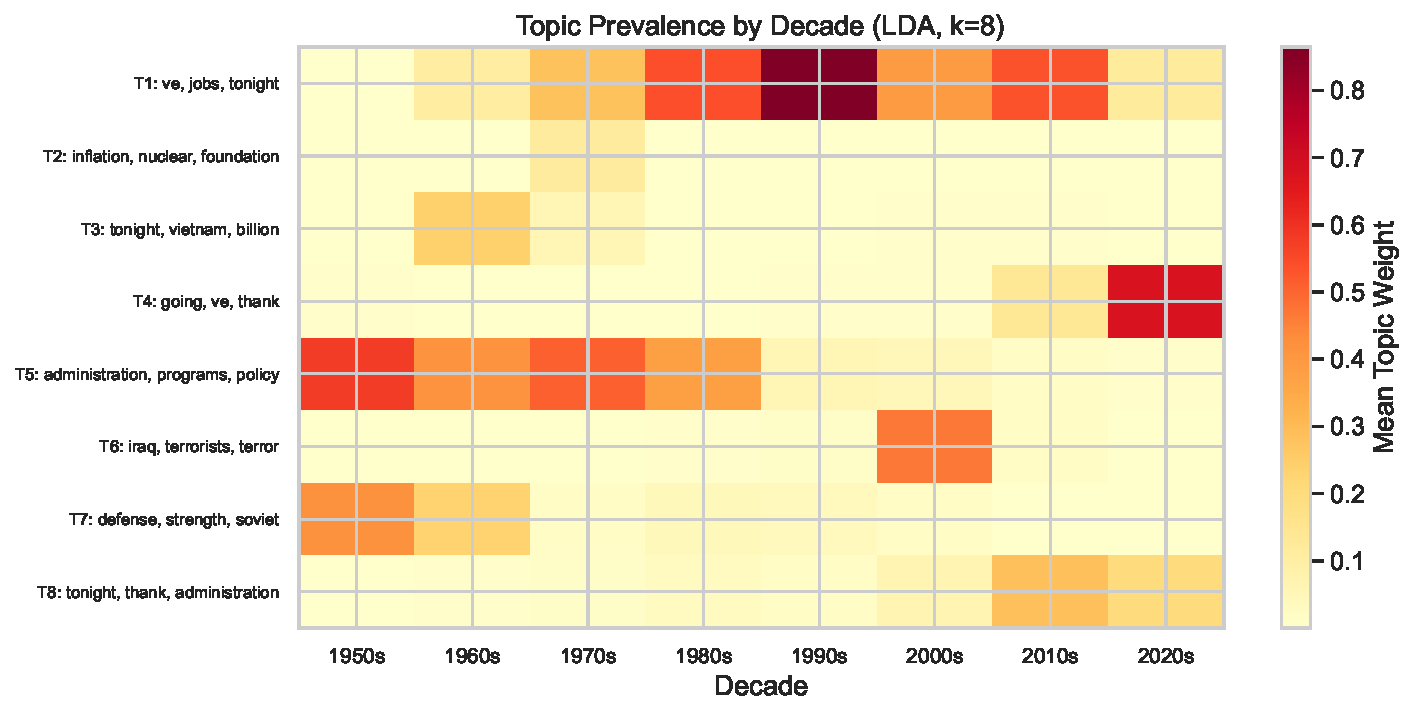
\includegraphics[width=\columnwidth]{figures/fig3a_topic_heatmap.pdf}
\caption{Mean topic prevalence by decade (LDA, $k=8$). Rows are topics labeled by top-3 words; columns are decades.}
\label{fig:topics_heat}
\end{figure}

In Figure~\ref{fig:topics_heat}, we see that topic prevalence changes dramatically over time. A topic dominated by \textit{defense, strength, soviet} concentrates in the 1950s and 1960s and fades sharply thereafter, once the early Cold War lexicon loses much of its referential grip. A topic centered on \textit{tonight, vietnam, billion} peaks in the 1960s and tapers off in the 1970s. The \textit{iraq, terrorists, terror} topic is very strongly localized to the 2000s. A bureaucratic topic of \textit{administration, programs, policy} dominates the mid-twentieth-century addresses (with weights between roughly 0.4 and 0.6 from the 1950s through the 1980s) and collapses in the 1990s. Finally, a topic featuring \textit{going, ve, thank} is essentially absent before the 2010s and rises sharply afterward, dominating the 2020s---capturing the shift toward conversational, audience-interactive rhetoric in the most recent SOTUs.

The overall trajectory can be described as a stratigraphy of American political language: from Cold War defense rhetoric, to Great Society programs, to post-Vietnam economic anxiety, to the War on Terror, and finally to the colloquial populism of the 2010s--2020s. As Nelson \citeyearpar{nelson2010} argues, topic models are best understood as ``starting points for interpretation''---guides to where close reading should begin.

\subsection{Supervised Classification}

Can a machine learning classifier predict the president's party from the text of a SOTU address? We tested four classifiers using 5-fold stratified cross-validation on TF-IDF features (3,000 features, unigrams and bigrams). Table~\ref{tab:classification} reports the results.

\begin{table}[h]
\centering
\small
\caption{Party Classification Accuracy (5-Fold CV)}
\label{tab:classification}
\begin{tabular}{lcc}
\toprule
\textbf{Model} & \textbf{Mean Acc.} & \textbf{Std.} \\
\midrule
Logistic Regression & 0.798 & 0.091 \\
Linear SVM & \textbf{0.924} & 0.061 \\
Random Forest & 0.823 & 0.060 \\
Gradient Boosting & 0.708 & 0.081 \\
\bottomrule
\end{tabular}
\end{table}

\begin{figure}[H]
\centering
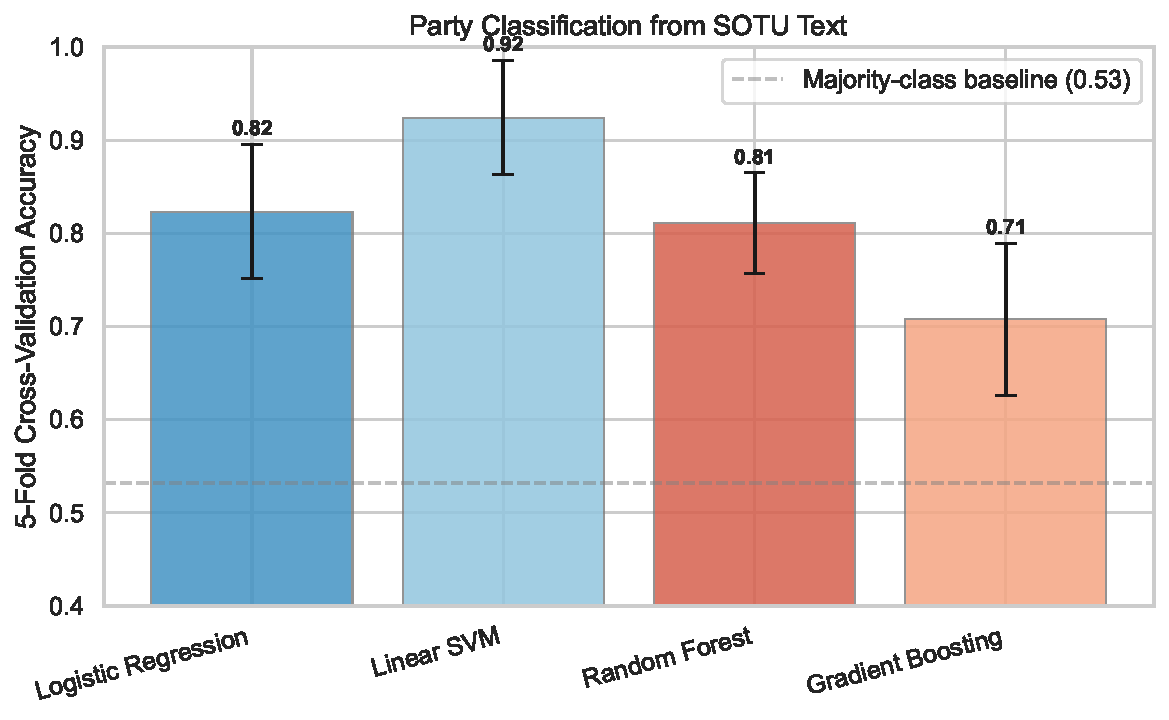
\includegraphics[width=0.85\columnwidth]{figures/fig4a_classification.pdf}
\caption{Classification accuracy across four models. Error bars show standard deviation across folds. Dashed line indicates the majority-class baseline (53\%, given 42/79 Republican speeches).}
\label{fig:classification}
\end{figure}

The Linear SVM achieves 92.4\% accuracy, substantially above the 53\% majority-class baseline. That a linear classifier operating on simple bag-of-words features can recover party affiliation at this rate is itself a non-trivial finding: it indicates that partisan vocabulary differences are not just real but largely separable in a high-dimensional sparse representation. This is consistent with So's \citeyearpar{so2017} observation that even imperfect models can be informative if their behavior is interpretable.

\subsection{Document Embedding Visualization}

To examine the global structure of the corpus without the mediation of a classifier, we projected all 79 speeches into two dimensions using TF-IDF features, dimensionality reduction via Truncated SVD (30 components), and t-SNE (perplexity=15).

\begin{figure}[H]
\centering
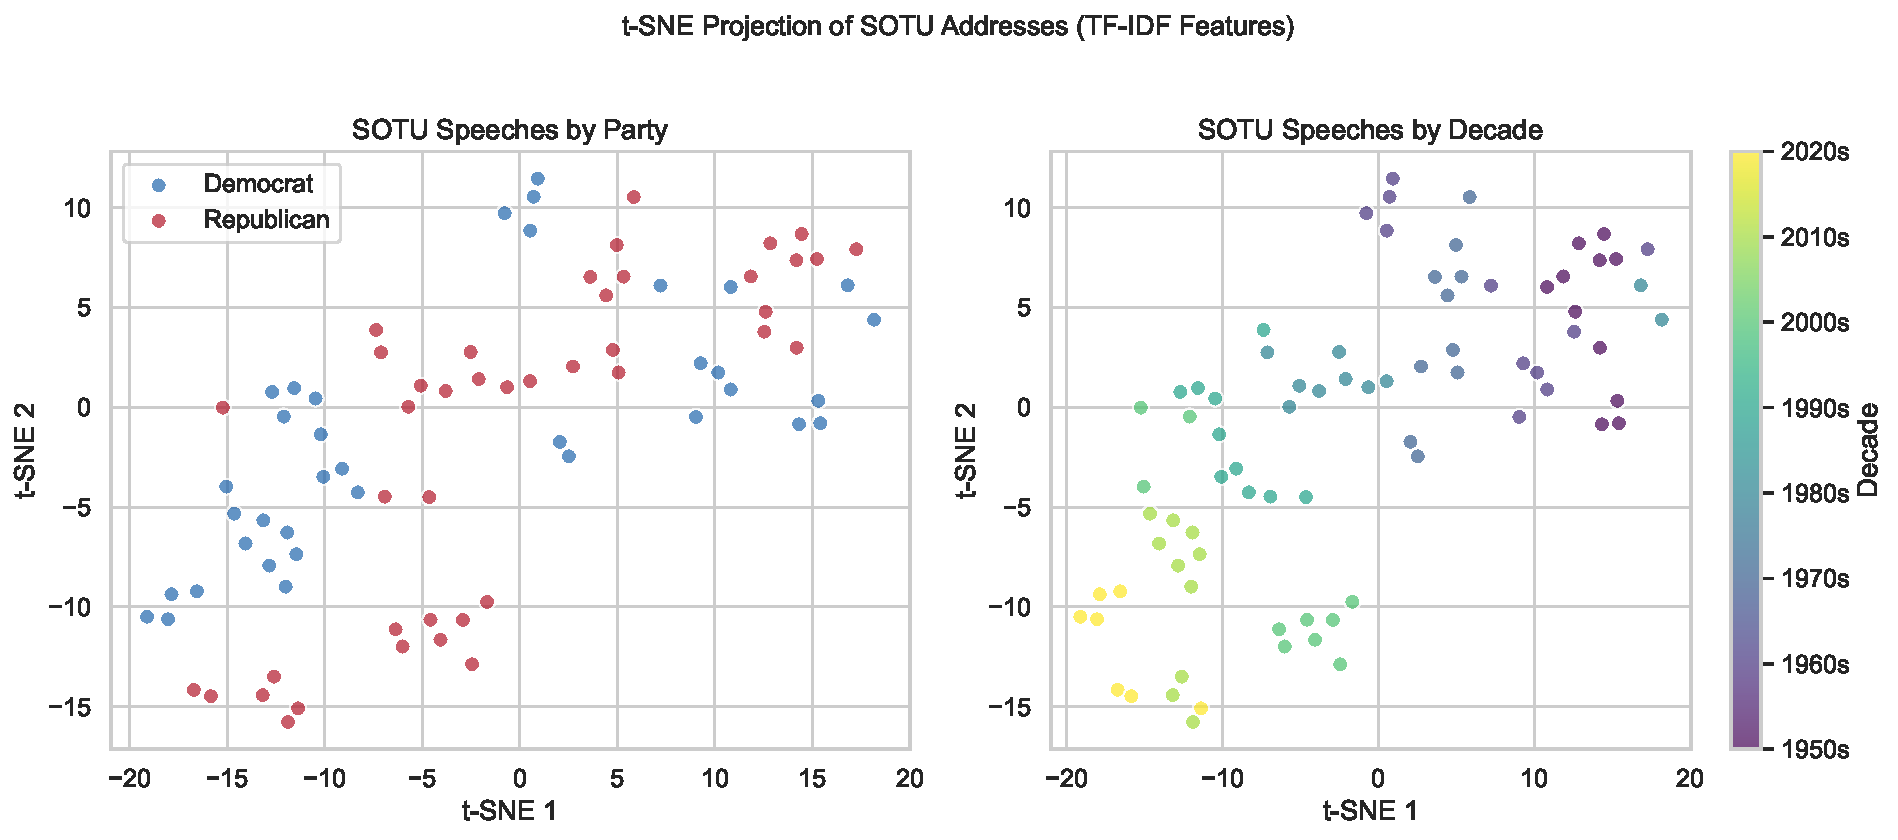
\includegraphics[width=\columnwidth]{figures/fig5_embeddings.pdf}
\caption{t-SNE projection of SOTU addresses. Left: colored by party. Right: colored by decade.}
\label{fig:embeddings}
\end{figure}

Figure~\ref{fig:embeddings} is perhaps the most revealing visualization in this paper. The left panel, colored by party, shows meaningful but imperfect clustering: Democratic and Republican speeches tend to occupy different regions of the space, but with substantial overlap. The right panel, colored by decade, tells a different story. Here the chronological gradient is unmistakable---1950s speeches in one region, 2020s speeches in another, with a smooth temporal progression in between. A Clinton speech sits closer to a George~W.\ Bush speech than to a Truman speech, because the shared linguistic context of the 1990s--2000s exerts a stronger gravitational pull than party affiliation.

These findings align with Underwood's \citeyearpar{underwood2019} argument that historical period routinely outweighs other categorical distinctions in large-scale text analysis---and suggests that models trained to detect partisanship may inadvertently be detecting periodization.

\subsection{Keyword Trends and Sentence Complexity}

We tracked the per-speech frequency of terms related to four thematic categories---security and defense, economy, social policy, and foreign policy---across the full corpus (Figure~\ref{fig:keywords}).

\begin{figure}[H]
\centering
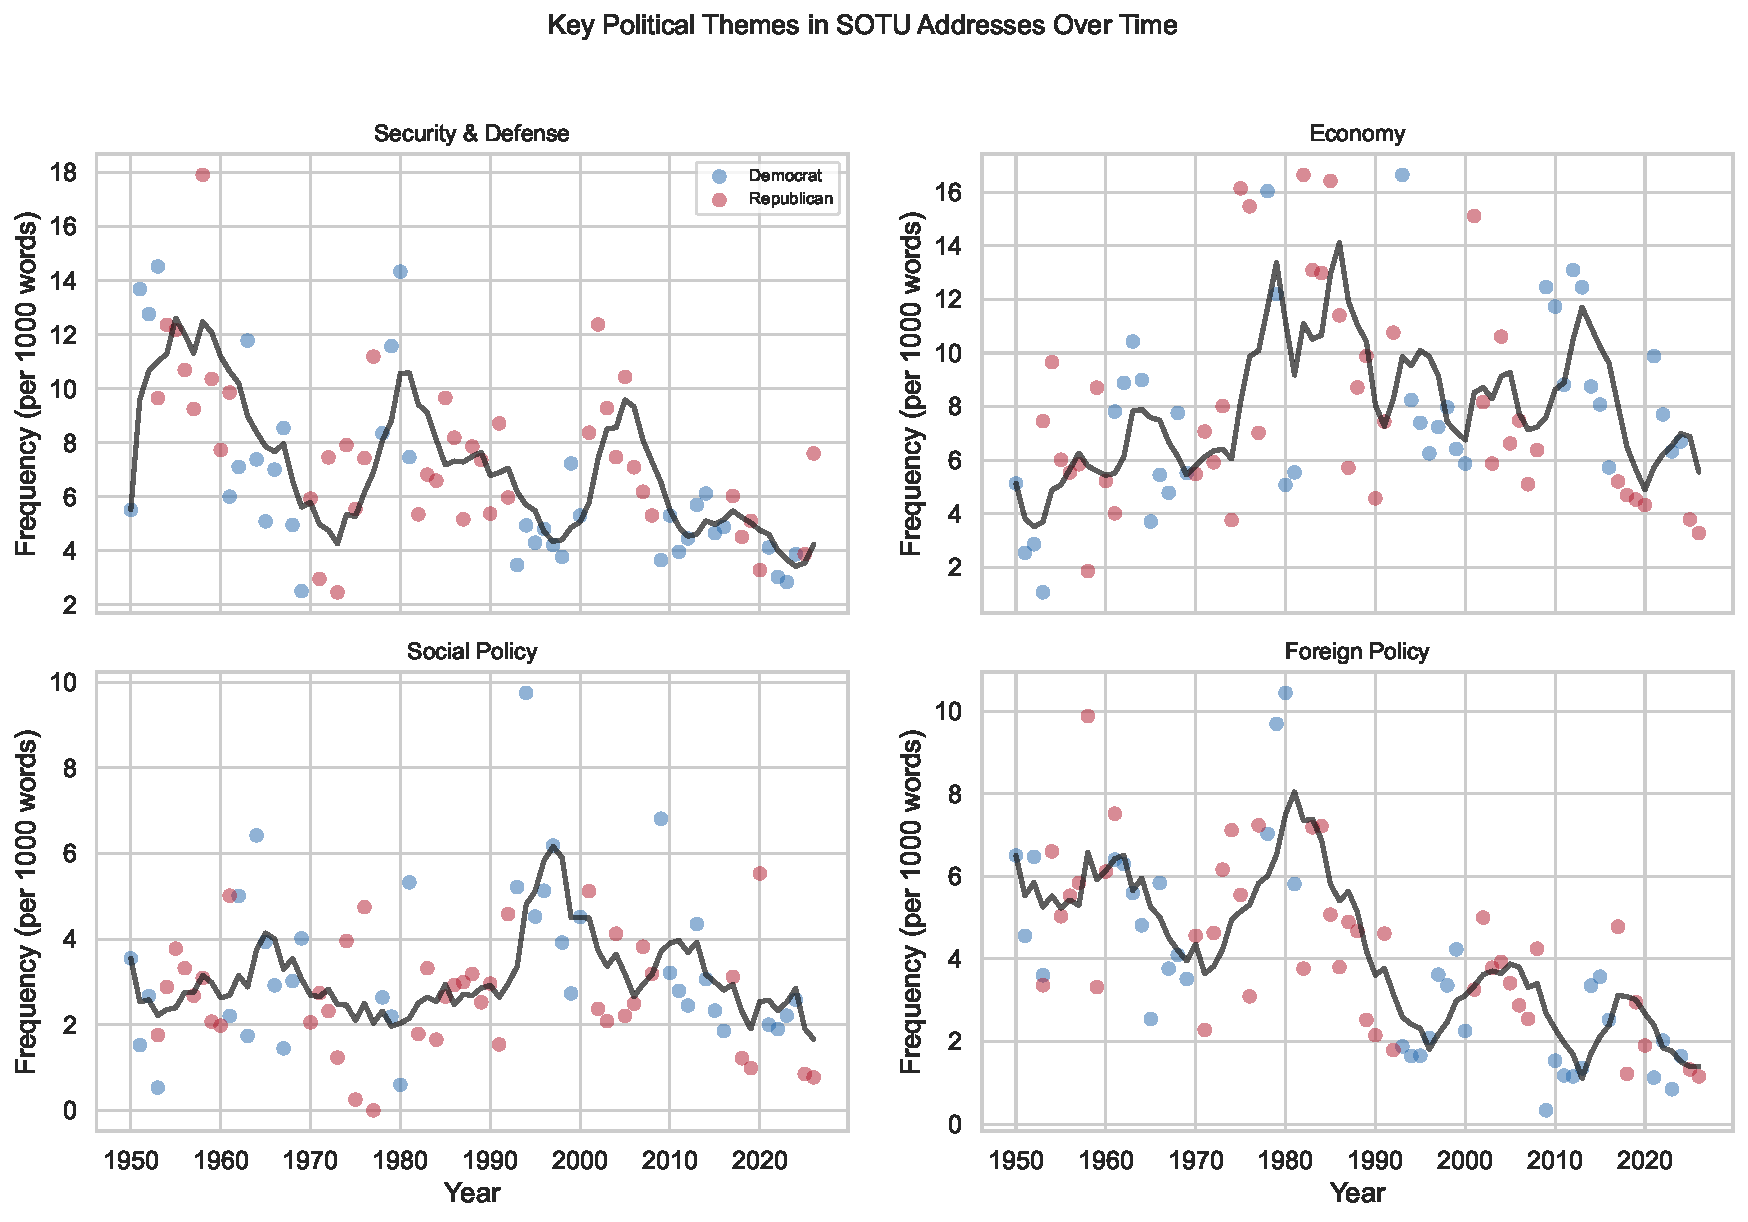
\includegraphics[width=\columnwidth]{figures/fig7_keyword_trends.pdf}
\caption{Frequency of key political terms (per 1,000 words) across four thematic domains, 1950--2026.}
\label{fig:keywords}
\end{figure}

The trends are historically interpretable. Defense and security language was at its highest frequency in the 1950s ($\approx 11.6$ per 1{,}000 words)---driven by the Korean War and the early Cold War---then dropped sharply in the 1960s, registered secondary peaks during the Reagan buildup of the 1980s and the post-9/11 years, and fell to its lowest corpus-wide values in the 2010s--2020s. Economic language rose continuously through the 1960s and 1970s, peaked across the late-Carter and Reagan years (the 1980s mean is the highest of any decade), and remained elevated through the Clinton, Obama, and post-2008 recovery years before declining in the 2020s. Social policy terms peaked in the Clinton 1990s, with secondary clusters in the George~W.\ Bush years; the Great Society addresses, perhaps surprisingly, register only moderate values on these keyword counts. Foreign policy language was broadly stable from the 1950s through the 1980s---hovering around five mentions per 1{,}000 words---then dropped sharply in the 1990s and continued to decline thereafter, reaching its lowest sustained values in the 2010s--2020s. This is a lexical trace of the turn toward domestic populism in both parties.

\begin{figure}[H]
\centering
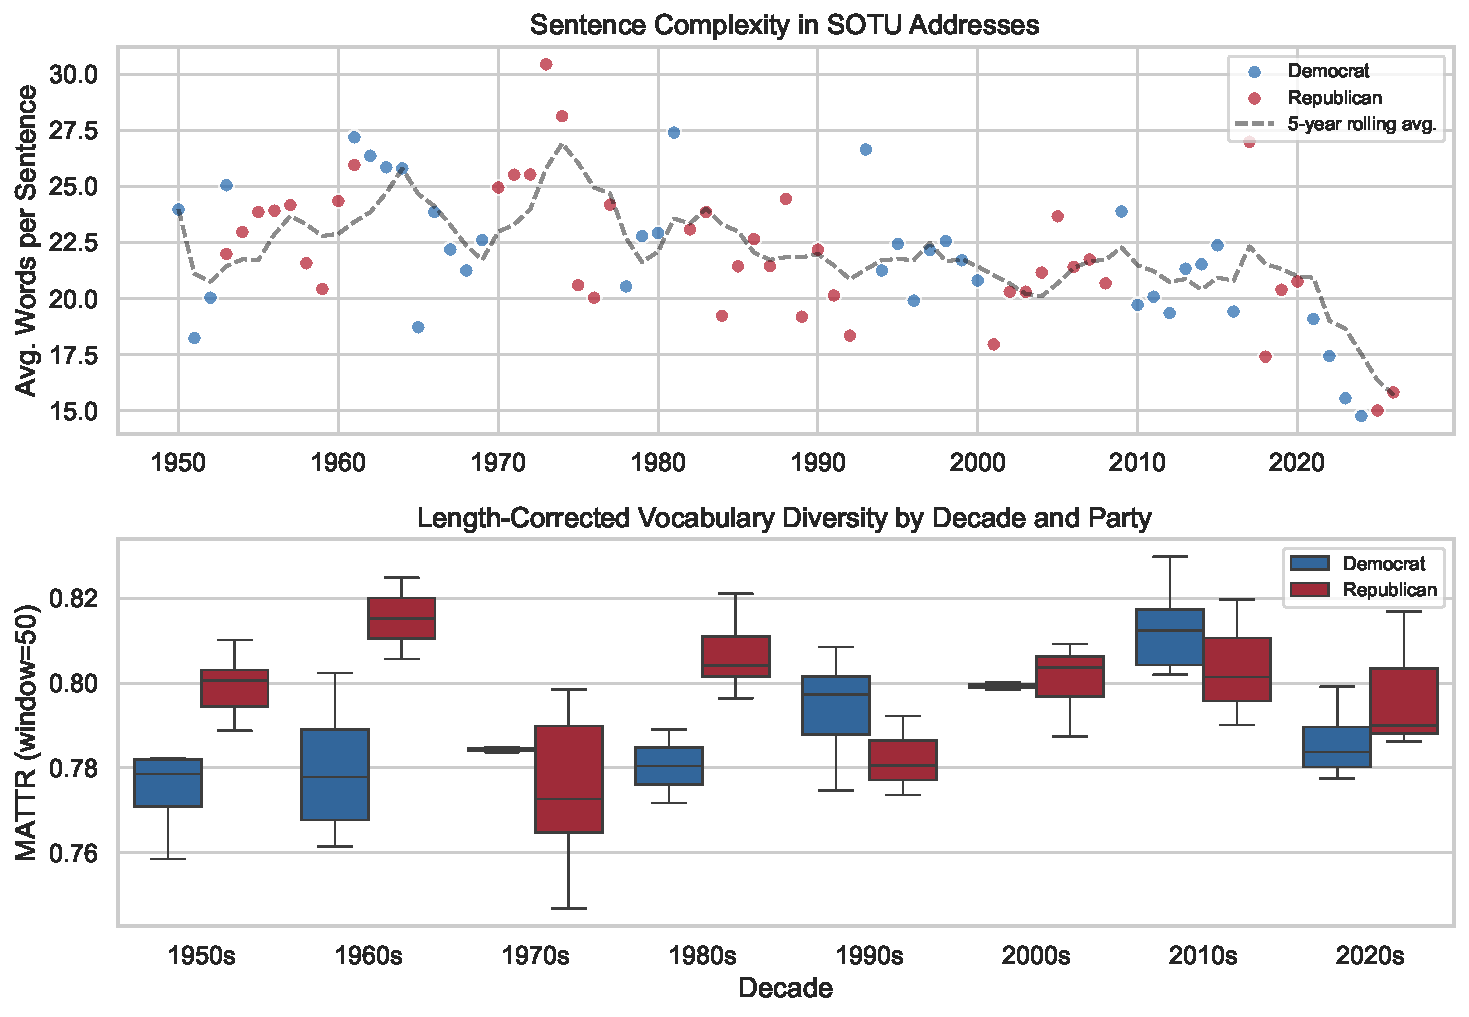
\includegraphics[width=\columnwidth]{figures/fig6_readability.pdf}
\caption{Sentence complexity (average words per sentence) and vocabulary diversity by decade and party.}
\label{fig:readability}
\end{figure}

Figure~\ref{fig:readability} examines sentence-level complexity. Average sentence length is essentially flat from the 1950s through the 1980s---hovering around 22--25 words per sentence---and then declines from the 1990s onward, falling to roughly 17 words per sentence in the 2020s. The inflection comes later than a conventional ``television revolution'' account would predict. The vocabulary diversity boxplots reveal a partisan pattern: Republican speeches sustain higher type-token ratios than Democratic ones in nearly every decade, with Democratic vocabulary diversity dropping noticeably from the 1980s onward.

% ===========================================================================
\section{Discussion}

Three important conclusions emerge from the analysis of SOTU speeches conducted here, each with implications for how we read political texts computationally.

\textbf{The dominance of the temporal signal.} Across every method used here---topic modeling, keyword tracking, t-SNE, and TF-IDF---historical period proved to be the main structuring force in SOTU rhetoric. The Cold War speeches of the 1950s are linguistically distant from the post-9/11 addresses of the 2000s, which are in turn distant from the populist rhetoric of the 2020s. As Sch\"och \citeyearpar{schoch2013} argues, ``big'' data in the humanities is also ``messy'' data: the temporal signal is entangled with every other variable we might want to isolate.

\textbf{Partisan signatures are real, but historically contingent.} The 92.4\% classification accuracy shows that Democratic and Republican presidents do use detectably different language. But the nature of that difference shifts across periods. The t-SNE projection (Figure~\ref{fig:embeddings}) suggests that 1950s--60s addresses cluster more by chronology than by party, while later speeches show somewhat greater partisan separation. Whether this represents a genuine widening of polarization or simply the entanglement of party with the distinctive lexicons of the post-9/11 and post-2020 periods is hard to disentangle without an ablation study comparing classification on early-only versus full-corpus subsets. We flag this as a question for future work.

\textbf{The limits of the bag of words.} Every analytical technique employed in this paper reduces SOTU speeches to distributions over terms, discarding syntax, rhetorical structure, and argumentative logic---the foundational trade-off of distant reading: scale for depth. As Drucker \citeyearpar{drucker2017} argues, the ``distant'' in distant reading is not merely spatial but epistemological. Perhaps the most productive use of these computational results is to identify \textit{where} close reading should focus: the moments where the model is most confident, or most confused.

\textbf{Limitations.} Our corpus, at 79 documents, is small by machine learning standards. SOTU addresses are also collaborative texts, so attributing patterns to individual presidents or parties requires caution. Future work might apply contextual embeddings such as BERT or adopt LLM-based topic evaluation methods \citep{yang2024}.

% ===========================================================================
\section{Conclusion}

Returning to the three questions we asked at the beginning: SOTU language has shifted dramatically across 1950--2026 in ways that track the historical pressures of each era; Democratic and Republican presidents do use detectably different vocabularies, though that boundary is permeable and historically contingent; and computational methods capture the broad architecture of these shifts well. The evidence supports the central argument: SOTU language is shaped more by the historical moment a president inhabits than by the party he carries into office.

% ===========================================================================
% References on a separate page
\bibliographystyle{apalike}
{\onecolumn
\bibliography{references}}

\end{document}